\documentclass[a4paper,12pt]{article}

\usepackage{amsmath,amssymb,amsthm,multicol,tikz,enumitem,diagbox,thmtools}
\usepackage{hyperref}
\usepackage{fancyvrb}
\usepackage[margin=2cm]{geometry}
\usetikzlibrary{calc}

\newcommand\N{\mathbf{N}}
\newcommand\Q{\mathbf{Q}}
\newcommand\R{\mathbf{R}}
\newcommand\Z{\mathbf{Z}}


\newcommand\indd{${}$\hspace{20pt}}

\declaretheoremstyle[headfont=\normalfont\bfseries,notefont=\mdseries\bfseries,bodyfont = \normalfont,headpunct={:}]{normalhead}
\declaretheorem[name={Uzdevums}, style=normalhead,numberwithin=section]{problem}

\setcounter{section}{101}

\setlength\parindent{0pt}





\begin{document}

{\Large \bf Uzdevums 25.2 (Pagrieziena matricas)}

\vspace{10pt}
{\bf Uzdevums 25.2} Plaknē dots trijstūris $\bigtriangleup{}ABC$ ar virsotnēm $A=A(x_A,y_A)$, $B=B(x_B,y_B)$, and $C = C(x_C,y_C)$. 
\begin{enumerate}
\item Pieņemsim, ka $\bigtriangleup{}ABC$ ir vienādmalu un divām virsotnēm $A,B$ ir veselas koordinātes 
($x_A,y_A,x_B,y_B \in \Z$). Pierādīt, ka tad $\bigtriangleup{}ABC$ laukums ir iracionāls. 
(Laukuma mērvienība ir vienas rūtiņas jeb vienības kvadrātiņa laukums.)
\item Pieņemsim, ka visām virsotnēm $A,B,C$ koordinātes ir veseli skaitļi. Pierādīt, ka 
šajā gadījumā $\bigtriangleup{}ABC$ laukums ir racionāls skaitlis.
\item Vai $\bigtriangleup{}ABC$ var būt vienādmalu trijstūris un visu virsotņu $A,B,C$ koordinātes
ir racionāli skaitļi? 
\end{enumerate}


{\em Ieteikums.} Apakšpunktā {\bf (B)} var izmantot Pīka teorēmu: \url{https://bit.ly/39m3qXH}.



\vspace{10pt}
{\bf (A)}\\
{\bf Pierādījums:} Apzīmēsim malas $AB$ garumu $|AB|$ ar $a$. Tā kā $x_A,y_A,x_B,y_B$ ir visi veseli, tad arī
$$|AB|^2 = (x_A - x_B)^2 + (y_A - y_B)^2 \in \Z.$$
(Šī vienādība seko no Pitagora teorēmas.) Zināms arī, ka vienādmalu trijstūra laukums, ja malas garums ir $a$ ir vienāds ar
\begin{equation}
\label{eq:triangle}
S_{\bigtriangleup{}ABC} = \frac{1}{2} a^2 \sin{}60^{\circ} = \frac{a^2 \sqrt{3}}{4}.
\end{equation}

\vspace{5pt}
Ievērosim, ka $\sqrt{3}$ ir iracionāls skaitlis.\\
Lai to pamatotu, pieņemsim, ka $\sqrt{3} = \frac{p}{q}$, kas ir nesaīsināma daļa un $p,q$ ir divi naturāli skaitļi, savstarpēji pirmskaitļi. 
Tad, kāpinot kvadrātā, $3q^2 = p^2$ un iegūstam, ka $p^2$ dalās ar $3$. Tāpēc $p$ arī dalās ar $3$ 
un to var izteikt $p = 3k$ kādam citam naturālam skaitlim $k$. 

Tad $3q^2 = (3k)^2 = 9k^2$ jeb $q^2 = 3k^2$. Iegūstam arī, ka $q^2$ dalās ar $3$. 
Tātad $p$ un $q$ abi dalās ar $3$; tas ir pretrunā ar pieņēmumu, ka 
ir nesaīsināma daļa, kas vienāda ar $\sqrt{3}$.

\vspace{5pt}
Pamatosim arī, ka reizinot racionālu skaitli $r \neq 0, r \in \Q$ ar iracionālu skaitli $\alpha \in \R -\Q$, reizinājums ir iracionāls.\\
Pieņemsim no pretējā, ka $r \cdot \alpha = r_1$, kur $r_1$ ir racionāls skaitlis.
Šajā gadījumā var izteikt $\alpha = r_1/r$, un tas būtu racionāls, kā divu racionālu skaitļu dalījums. 
Tas ir pretrunā ar pieņēmumu, ka $\alpha$ ir iracionāls.


\vspace{5pt} 
Atgriežamies pie vienādojuma (\ref{eq:triangle}).\\
$S_{\bigtriangleup{}ABC}$ ir reizinājums
racionālam $\frac{a^2}{4} = \frac{(x_A - x_B)^2 + (y_A - y_B)^2}{4}$ ar iracionālu skaitli $\sqrt{3}$. 
To reizinājumam jābūt iracionālam. $\blacksquare$



\vspace{10pt}
{\bf (B)}\\
{\bf Pierādījums:} Pieņemsim, ka $\bigtriangleup{}ABC$ visas koordinātes ir veseli skaitļi. 
Izmantosim Pīka teorēmu: Tā kā $ABC$ ir vienkāršs daudzstūris (tā iekšienē nav caurumu un malas 
cita citu nekrusto), tad tā laukums ir $S_{\bigtriangleup{}ABC} = i + \frac{b}{2} - 1$, kur $i$ ir iekšējo punktu skaits ar veselām koordinātēm (turpmāk 
sauktas ``rūtiņu virsotnes''), un
$b$ ir ``rūtiņu virsotņu'' skaits uz figūras robežas. 
Tāpēc laukums šādam trijstūrim vienmēr būs vai nu vesels skaitlis vai vesels skaitlis plus $1/2$. 
Tādēļ tam vienmēr jābūt racionālam. 

Ja nevēlaties izmantot Pīka teorēmu, apvelciet pa rūtiņu līnijām taisnstūri ap $ABC$. 
Taisnstūrim ir vesels laukums, un $S_{\bigtriangleup{}ABC}$ var iegūt, atņemot no tā dažu taisnleņķa
trijstūru laukumus (ar abām veselām katetēm).\\
Attēls~\ref{fig:grid-triangles} parāda abas metodes, kā rēķināt laukumu. Pēc Pīka teorēmas šajā piemērā:
$$S_{\bigtriangleup{}ABC} = 16 + \frac{4}{2} - 1 = 17.$$
Atņemot pelēkos trijstūrus:
$$S_{\bigtriangleup{}ABC} = S_{CKLM} - S_{CKA} - S_{ALB} - S_{BMC} = 42 - \frac{7 \cdot 4}{2} - \frac{2 \cdot 5}{2} - \frac{6 \cdot 2}{2} = 17.$$

\begin{figure}[!htb]
\center{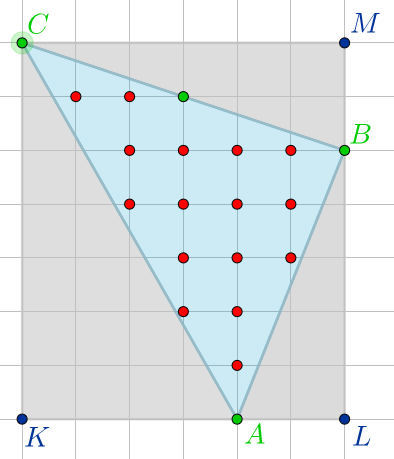
\includegraphics[width=2in]{hw02-5/25-2-grid-triangles.png}}
\caption{\label{fig:grid-triangles} Trijstūris $ABC$ ar visām veselu skaitļu virsotnēm.}
\end{figure}






\vspace{10pt}
{\bf (C)}\\
{\bf Apgalvojums.} Neeksistē vienādmalu trijstūris $ABC$ ar visām racionālām koordinātēm. 

{\bf Pierādījums.} Pieņemsim, ka vienādmalu trijstūrim
$\bigtriangleup{}ABC$ visu virsotņu koordinātes $x_A$, $y_A$, $x_B$, $y_B$, $x_C$, $y_C$ in $\Q$ 
($\Q$ ir racionālo skaitļu kopa). 
Visiem sešiem skaitļiem ir saucēji \textendash{} apzīmējam tos ar $q_1,q_2,q_3,q_4,q_5,q_6$. 
Pareizināsim visas $ABC$ koordinātes ar $q_1 \cdot q_2\cdot q_3\cdot q_4\cdot q_5\cdot q_6$. 
Pēc pārveidojuma (homotētija ar centru koordinātu sākumpunktā) trijstūris
joprojām ir vienādmalu, bet tā visu virsotņu koordinātes ir jau veseli skaitļi. 

Kā uzzinājām apakšpunktā {\bf (A)}, $\bigtriangleup{}ABC$ ar veselām koordinātēm laukums ir iracionāls. 
Bet saskaņā ar {\bf (B)}, trijstūra $\bigtriangleup{}ABC$ laukumam jābūt racionālam, jo visas tā virsotnes ir veseli skaitļi. 
Laukums $S_{\bigtriangleup{}ABC}$ nevar būt vienlaikus racionāls un iracionāls. Iegūta pretruna un tātad šāds trijstūris neeksistē.
$\blacksquare$


\vspace{20pt}
{\bf Par pagrieziena matricām}

Šī piebilde nav vajadzīga uzdevuma risināšanā, bet ir svarīga tiem, kuri apgūst lineāro algebru un matricas. 
Ir iespējams uzzīmēt trijstūrus, kam visas virsotnes ir veseli skaitļi un 
kas ir ļoti ``tuvi'' vienādmalu trijstūriem (bet nav vienādmalu).
Sk.\ Attēlu~\ref{fig:approximate-triangle} \textendash{} tajā punkti $A(0;0)$ un
$B(15,4)$, un $C(4,15)$ visi ir ar veselām koordinātēm.

Savukārt, ja mēģināsim iegūt trešo punktu $C$, pagriežot taisnes nogriezni $AB$ pretēji pulksteņa rādītājiem par $60^{\circ}$ 
ap punktu $A(0;0)$, 
tad $C$ koordinātes var iegūt, izmantojot {\em pagrieziena matricu} ({\em Rotation matrix}; \url{https://bit.ly/3pc1c3F}). 

\[ \left( \begin{array}{c}
x_C \\
y_C \\
\end{array} \right) = \left(
%\arraycolsep=1.4pt\def\arraystretch{2.2}
\begin{array}{ll} 
\cos \alpha & -\sin \alpha \\ 
\sin \alpha  & \cos \alpha \\ 
\end{array} \right) \cdot \left(
\begin{array}{c}
x_B \\
y_B \\
\end{array} \right). \]

Aprēķināsim virsotnes $C$ koordinātes, ievietojot $x_B = 15$, $y_B = 4$, un $\alpha = 60^{\circ} = \frac{\pi}{3}$. 

\[ \left\{ \begin{array}{l}
x_C = x_B \cdot \cos \alpha - y_B \cdot \sin \alpha = 15 \cdot \frac{1}{2} - 4 \cdot \frac{\sqrt{3}}{2} = 4.035898384862247\ldots{}, \\
y_C = x_B \cdot \sin \alpha + y_B \cdot \cos \alpha = 15 \cdot \frac{\sqrt{3}}{2} + 4 \cdot \frac{1}{2} = 14.990381056766578\ldots{}. \\
\end{array} \right.
\]

Šajā gadījumā $C$ ir iracionālas koordinātes (pat ja šajā un līdzīgos piemēros var panākt, lai tās būtu cik patīk tuvu veseliem skaitļiem). 
Un trijstūra $\bigtriangleup{}ABC$ laukums ir iracionāls. 


\begin{figure}[!htb]
\center{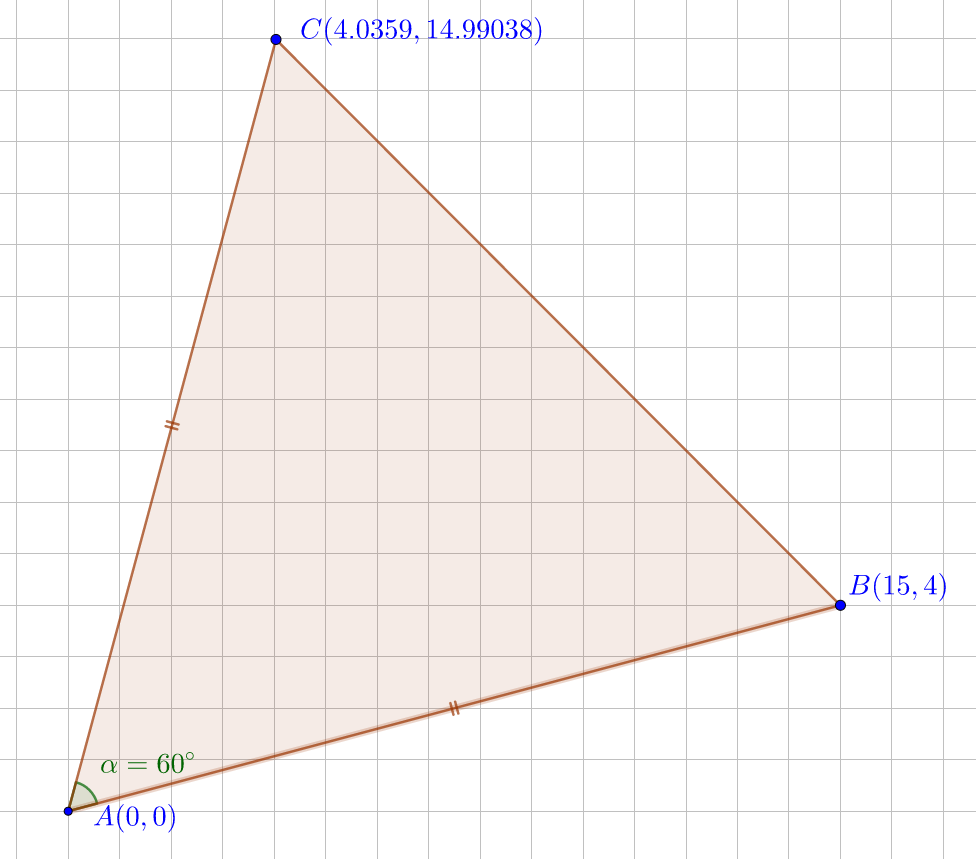
\includegraphics[width=3in]{hw02-5/25-2-approximate-triangle.png}}
\caption{\label{fig:approximate-triangle} Vienādmalu $\bigtriangleup{}ABC$, kam  $C$ koordinātes noapaļotas līdz $5$ cipariem.}
\end{figure}





\end{document}